\documentclass[]{book}

% QCC book needs
\usepackage{fix-cm}  % this package allows large \fontsize
\usepackage{imakeidx}
\makeindex[title=Index]
\usepackage{listings}
\usepackage[table]{xcolor}

\usepackage{amsmath,graphicx}

\usepackage{tikz}    % this is for graphics. e.g. rectangle on title 
\usetikzlibrary{quantikz, decorations.pathmorphing,shapes.geometric}
%\usepackage{circuitikz}
\usepackage{tikz-3dplot} % includes tikz
\tdplotsetmaincoords{70}{120}
\usepackage{float}


% This file is for commands / macros / functions.
% QCC book specific
\newcommand{\keta}[2][]{\vert {#2} \rangle_{#1}}
\newcommand{\braketa}[3][]{\langle {#2} \vert {#3}\rangle_{#1}}

\tikzstyle{Gate}=[rectangle, minimum width=30, minimum height=30, text width=20, text centered, draw=black]
\usepackage{pgfplots}
\usepgfplotslibrary{fillbetween}

\begin{document}

%\label{Demodulator-QP}
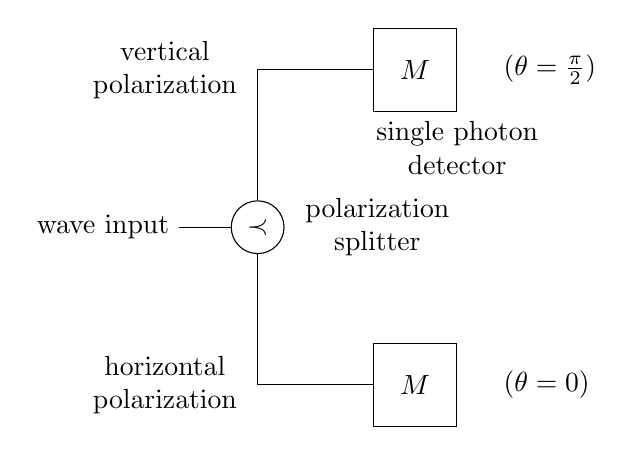
\begin{tikzpicture}[scale=1]
    \path
    (-3,0) node[anchor=east] (input) {wave input}
    (-2,0) node[circle, draw=black] (split) {$\prec$}
    (0,2) node[Gate] (tsp) {$M$}
    (0,-2) node[Gate] (bsp) {$M$};
     
    \path 
    (-2,2) node [text width=60, align=center, anchor=east] (V) {vertical polarization}
    (-2,-2) node [text width=60, align=center, anchor=east] (H) {horizontal polarization}
    (1,2) node [anchor=west] (bit01) {$(\theta=\frac \pi 2)$}
    (1,-2) node [anchor=west] (bit00) {$(\theta=0)$};

    \draw (input) -- (split) |- (tsp);
    \draw (split) |- (bsp);
    \draw (split.east) node[text width=60, align=center, anchor=west] {polarization splitter};
    \draw (tsp.south east) node[text width=60, align=center, anchor=north] {single photon detector};
\end{tikzpicture}

%\label{Demodulator-DP2}
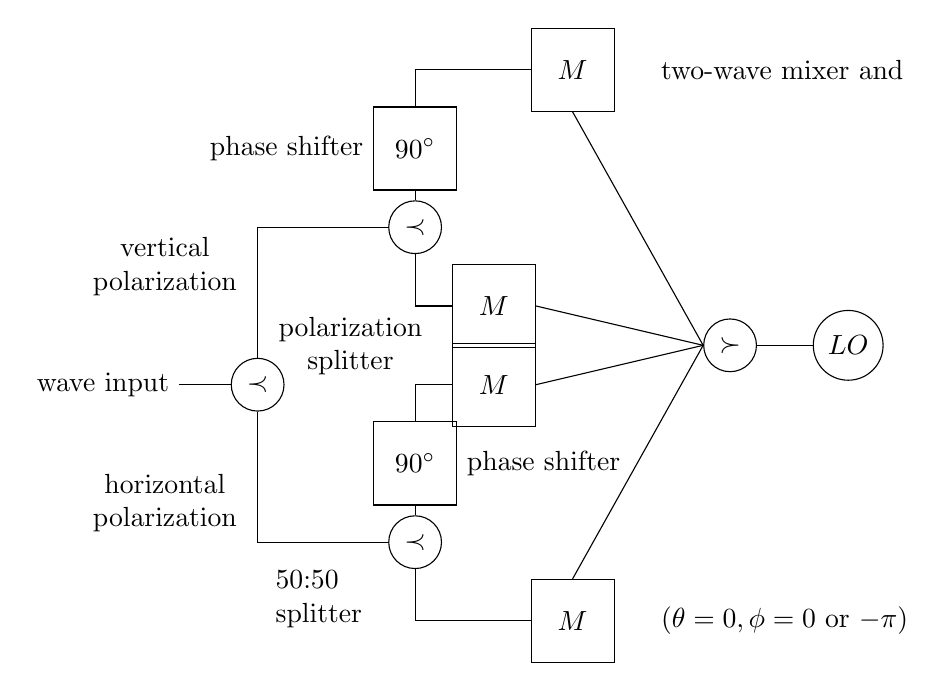
\begin{tikzpicture}[scale=1]
    \path
    (-3,0) node[anchor=east] (input) {wave input}
    (-2,0) node[circle, draw=black] (split) {$\prec$}
    (0,2) node[circle, draw=black] (tsp) {$\prec$}
    (0,-2) node[circle, draw=black] (bsp) {$\prec$}
    (0,3) node[Gate] (tphi90) {$90^\circ$}
    (0,-1) node[Gate] (bphi90) {$90^\circ$}
    (2,4) node[Gate] (td1) {$M$}
    (1,1) node[Gate] (td2) {$M$}
    (1,0) node[Gate] (bd1) {$M$}
    (2,-3) node[Gate] (bd2) {$M$}
    (4,0.5) node[circle, draw=black] (gg) {$\succ$}
    (5.5,0.5) node[circle, draw=black] (lo) {$LO$};

    \path (3,4) node[anchor=west] (bit11) {two-wave mixer and }
    (3,-3) node [anchor=west] (bit00) {$(\theta=0, \phi=0$ or $-\pi)$}
    (-2,1.5) node [text width=60, align=center, anchor=east] (V) {vertical polarization}
    (-2,-1.5) node [text width=60, align=center, anchor=east] (H) {horizontal polarization};
%    (2,1) node [anchor=west] (bit10) {$(\theta=\frac \pi 2, \phi=$0 or $-\pi)$}
%    (2,0) node [anchor=west] (bit01) {$(\theta=0, \phi=\frac \pi 2$ or $-\frac \pi 2)$}

    \draw (input) -- (split) |- (tsp) -- (tphi90) |- (td1);
    \draw (split) |- (bsp) -- (bphi90) |- (bd1);
    \draw (tsp) |- (td2);
    \draw (bsp) |- (bd2);
    \draw (gg.west) -- (td1.south);
    \draw (gg.west) -- (td2.east);
    \draw (gg.west) -- (bd1.east);
    \draw (gg.west) -- (bd2.north);
    \draw (gg) -- (lo);
    \draw (split) node[text width=60, align=center, anchor=south west] {polarization splitter};
%    \draw (tsp.south west) node[text width=40, anchor=north east] {50:50 splitter};
    \draw (bsp.south west) node[text width=40, anchor=north east] {50:50 splitter};
    \draw (tphi90.west) node[anchor=east] {phase shifter};
    \draw (bphi90.east) node[anchor=west] {phase shifter};
%    \draw (td1.south east) node[text width=60, align=center, anchor=north west] {single photon detector};
\end{tikzpicture}

%\label{Demodulator}
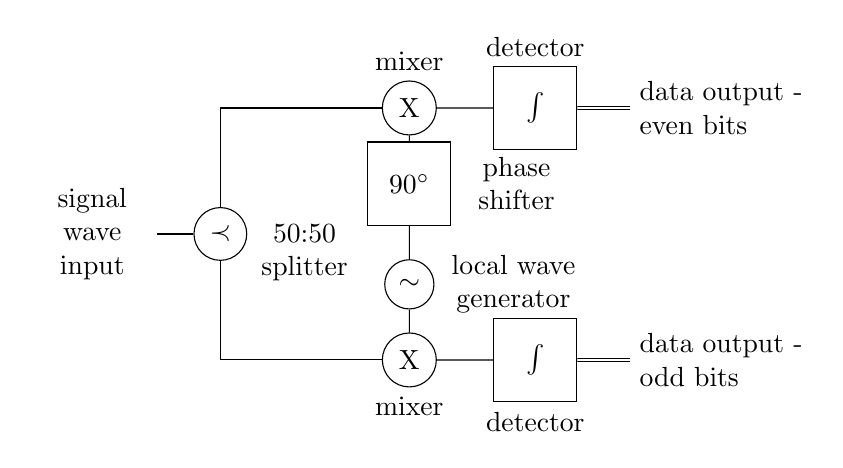
\begin{tikzpicture}[scale=0.8]
    \path
    (0,-0.8) node[circle, draw=black] (lo) {$\sim$}
    (0,0.8) node[Gate] (p90) {$90^\circ$}
    (0,2) node[circle, draw=black] (ta) {X}
    (0,-2) node[circle, draw=black] (ba) {X}
    (2,2) node[Gate] (tm) {$\int$}
    (2,-2) node[Gate] (bm) {$\int$}
    (-3,0) node[circle, draw=black] (split) {$\prec$}
     (-4,0) node[text width=40, align=center, anchor=east] (input) {signal wave input};
    \path (3.5,2) node[text width=60, align=left, anchor=west] (even) {data output - even bits}
    (3.5,-2) node [text width=60, align=left, anchor=west] (odd) {data output - odd bits};

    \draw (lo.east) node[text width=50, align=center, anchor=west] {local wave generator};
    \draw (p90.east) node[text width=40, align=center, anchor=west] {phase shifter};
    \draw (tm.north) node[anchor=south] {detector};
    \draw (bm.south) node[anchor=north] {detector};
    \draw (ta.north) node[anchor=south] {mixer};
    \draw (ba.south) node[anchor=north] {mixer};
    \draw (bm) -- (ba) -- (lo) -- (p90) -- (ta) -- (tm);
    \draw[double] (even) -- (tm);
    \draw[double] (odd) -- (bm);

    \draw (ba) -| (split)  |- (ta);
    \draw (split.south east) node[text width=40, align=center, anchor=west] {50:50 splitter};
    \draw (split) -- (input);    
\end{tikzpicture}

%\label{Demodulator-DP-QPSK}
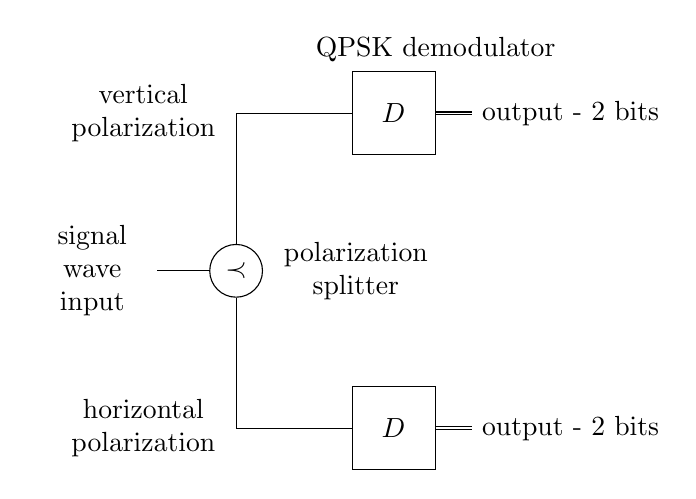
\begin{tikzpicture}[scale=1]
    \path
    (-3,0) node[text width=40, align=center, anchor=east] (input) {signal wave input}
    (-2,0) node[circle, draw=black] (split) {$\prec$}
    (0,2) node[Gate] (tsp) {$D$}
    (0,-2) node[Gate] (bsp) {$D$};
     
    \path 
    (-2,2) node [text width=60, align=center, anchor=east] (V) {vertical polarization}
    (-2,-2) node [text width=60, align=center, anchor=east] (H) {horizontal polarization}
    (1,2) node [anchor=west] (bit01) {output - 2 bits}
    (1,-2) node [anchor=west] (bit00) {output - 2 bits};

    \draw[double] (tsp) -- (bit01);
    \draw[double] (bsp) -- (bit00);
    
    \draw (input) -- (split) |- (tsp);
    \draw (split) |- (bsp);
    \draw (split.east) node[text width=60, align=center, anchor=west] {polarization splitter};
    \draw (tsp.north east) node[anchor=south] {QPSK demodulator};
\end{tikzpicture}

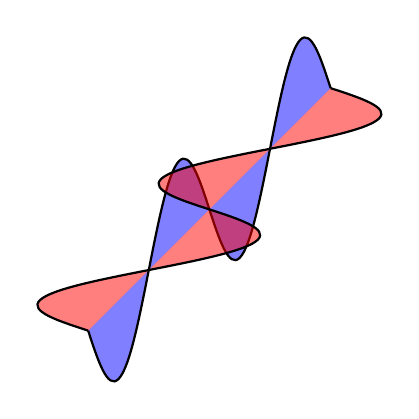
\begin{tikzpicture}%[z={(10:10mm)},x={(-45:5mm)}]
  \def\wave{
    \draw[fill,thick,fill opacity=0.5]
     (0,0) sin (1,1) cos (2,0) sin (3,-1) cos (4,0)
           sin (5,1) cos (6,0) sin (7,-1) cos (8,0);
           %sin (9,1) cos (10,0)sin (11,-1)cos (12,0);
%    \foreach \shift in {0,4,8}
%    {
%      \begin{scope}[xshift=\shift cm,thin]
%        \draw (.5,0)  -- (0.5,0 |- 45:1cm);
%        \draw (1,0)   -- (1,1);
%        \draw (1.5,0) -- (1.5,0 |- 45:1cm);
%        \draw (2.5,0) -- (2.5,0 |- -45:1cm);
%        \draw (3,0)   -- (3,-1);
%        \draw (3.5,0) -- (3.5,0 |- -45:1cm);
%      \end{scope}
%    }
  }
  \begin{scope}[canvas is zy plane at x=0,fill=blue]
    \wave
%    \node at (6,-1.5) [transform shape] {magnetic field};
  \end{scope}
  \begin{scope}[canvas is zx plane at y=0,fill=red]
%    \draw[help lines] (0,-2) grid (12,2);
    \wave
%    \node at (6,1.5) [rotate=180,xscale=-1,transform shape] {electric field};
  \end{scope}
\end{tikzpicture}

\end{document}